%\section{System Model and Problem Formulation}
\section{Preliminaries}
\label{sectionmodel}

In this section, we first give some notion definitions and introduce the collision detection mechanism. 
Then we formulate the Neighbor Discovery problem formally.  


\subsection{Sensor Node Model}

The wireless sensor network consists of a number of sensors distributed separately in a target area.
The deployed sensor nodes keep their most time in sleep pattern to avoid quick energy consumption 
and wake up timely to work on duty.

In our model, we assume that each node has a unique identifier $ID_i$ which is aware by theirselves, while the total amount of sensors $N$  is not necessary to be known. Time is divided into slots of equal length $t_0$, 
which is sufficient to finish  one communication process(transmit or receive a piece of package). In each time slot, a node transform its pattern according to a pre-defined duty schedule.

\begin{definition}
\textbf{Duty schedule} is a pre-defined sequence $S=\{s^t\}_{0\leq t<T}$ of period $T$ and
$$ s^t=\left\{
\begin{aligned}
0  & & & {sleep}\\
1  & & & {wake-up}\\
\end{aligned}
\right.
$$
\end{definition}

 Each node construct its own duty schedule according to a specific strategy and repeats it
 until finding all the neighbors. Since the waking-up duration has a significant affect on the battery's lifetime, 
 duty circle is defined to restrict the energy consumption.

\begin{definition}
\textbf{Duty circle} represents the fraction of one period T where a node turns its radio on. It can be formulated as:

$$\theta=\frac{|\{ 0\leq t<T : s^t =1\}}{T}.
$$
  
\end{definition}

When a sensor wake up on a time slot, it can turn to either the transmitting state or listening state. 
\begin{itemize}
\item \textbf{Transmitting state}. A node turn to transmitting state will broadcast a package containing its own identify 
information to all neighbors.
\item  \textbf{Listening state}. A node turn to listening state will monitor the frequency channel to collect its neighbors' packages.
However collision will occur when two or more neighbor nodes transmit concurrently and thus no valid information will be gathered
\end{itemize}
Transiting between the states only costs little time, compared to one complete time slot.

%@@@ to be modified
\subsection{Collision Detection Mechanism}

A collision detection mechanism allows a node to distinguish between 
the case where two or more nodes are transmitting and one where no 
node is transmitting. Indeed, practical solutions for collision detection 
have been proposed in [5, 6]. In this paper, we study two neighbor 
discovery algorithms, first when nodes do not have a collision detection 
mechanism and next when nodes do and study the impact of collision 
detection on algorithm performance.

%@@@




\subsection{Problem Definition}

We consider a partially-connected sensor network, 
where two nodes are neighbors if they locate within the radio range of each other. 
A  symmetric matrix $M_{N\times N}$ is used to record the neighboring relations as:

$$ M_{i,j}=\left\{
\begin{aligned}
1  & & & & & & {connected}\\
0  & & & & & & {disconnected}\\
\end{aligned}
\right.
$$

Each sensor follows its duty schedule to achieve neighbor discovery. In a synchronous scenario,
sensors start their neighbor discovery process at the same time, while in a asynchronous  scenario
all nodes start at different time slots.
 
Notice that the neighbor discovery process is not bidirectional, which means any pair of neighbors 
need to find each other separately. The time slots within which a sensor node $u_i$ find one of its neighbors $u_j$ can be formulated 
as $L(i,j)$. Then we define the discovery latency that node $u_i$ discovers all neighbors as:

\begin{definition}
\textbf{Discovery latency} of node $u_i$ is the time to discover all neighbors:
$$L(i) = \max_{M_{i,j = 1}} L (i,j).
$$
\end{definition}

Thus the neighbor discovery problem can be formulated as:
%@@@to be modified
\begin{problem}
Given a duty circle $\theta$, design a duty schedule and transiting strategy which optimizes $L(i)$ to the most extent. 
\end{problem}
%@@@

\begin{figure}[!t]
\centering
\subfigure[Topology]{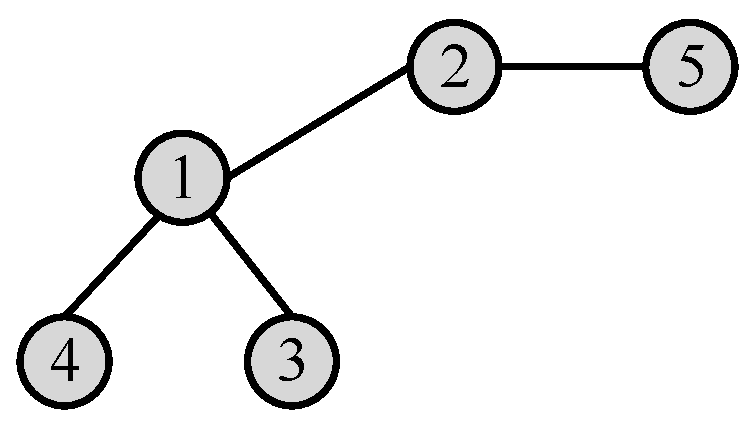
\includegraphics[width=1.65in]{./Figure/topology.eps}}
\vspace{0.03in}
\subfigure[Neighbor discovery process]{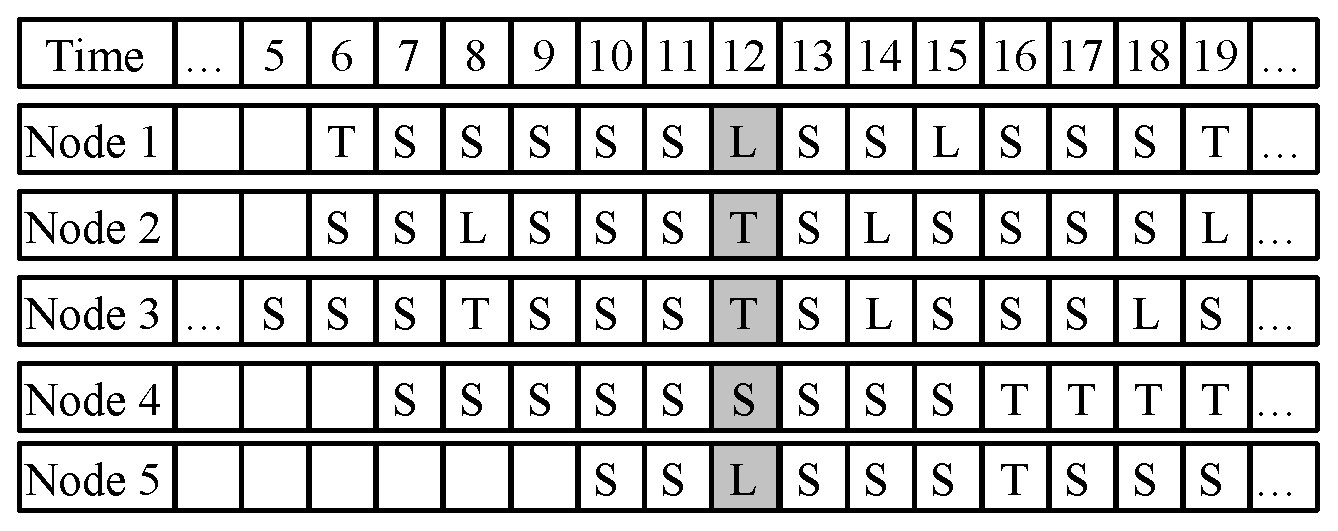
\includegraphics[width=2.8in]{./Figure/NBexample.eps}}
\caption{An example of neighbor discovering process. S, T and L represents Sleep pattern, 
Transmitting state and Listening state in wake-up pattern.}
\label{NDexample}
%\vspace{-0.2in}
\end{figure}

An example of neighbor dicovery process is given in Fig.\ref{NDexample}. 
Fig.\ref{NDexample}(a) shows the topology of a partially-connected 
wireless sensor networks, which consists of $5$ sensor nodes. 
Fig.\ref{NDexample}(b) describes the neighbor discovery process 
in the asynchronous scenario, as we can see the nodes 
start their process at different time slot. The duty schedule of 
node $1$, for example, is $S_1=\{1,0,0,0,0,0,1,0,0,1,0,0,0,1,...\}$.  
At time slot $12$, node 5 find its neighbor node $2$ while node $1$ 
could not find node $2$ due to a collision from its another neighbor node $3$. 



